%%%%%%%%%%%%%%%%%%%% author.tex %%%%%%%%%%%%%%%%%%%%%%%%%%%%%%%%%%%
%
% sample root file for your "contribution" to a proceedings volume
%
% Use this file as a template for your own input.
%
%%%%%%%%%%%%%%%% Springer %%%%%%%%%%%%%%%%%%%%%%%%%%%%%%%%%%


\documentclass{svproc}
%
% RECOMMENDED %%%%%%%%%%%%%%%%%%%%%%%%%%%%%%%%%%%%%%%%%%%%%%%%%%%
%

% to typeset URLs, URIs, and DOIs
\usepackage{bm,color,mathtools,graphicx,url}
\def\UrlFont{\rmfamily}

\setlength{\tabcolsep}{5pt}
\newcommand{\unit}[2]{#1\,#2}
%\newcommand{\reva}[1]{{\color{blue}#1}}
\newcommand{\reva}[1]{{\color{black}#1}}
%\newcommand{\revb}[1]{{\color{red}#1}}
\newcommand{\revb}[1]{{\color{black}#1}}
\renewcommand{\arraystretch}{1.5}

\begin{document}
\mainmatter % start of a contribution
%
\title{Application of smoothed particle hydrodynamics to a ballistic gelatine sample high-speed impact}
%
\titlerunning{Smoothed particle hydrodynamics}  % abbreviated title (for running head) also used for the TOC unless \toctitle is used
%
\author{Lud\v{e}k Hyn\v{c}\'{\i}k\inst{1}}
%
\authorrunning{Lud\v{e}k Hyn\v{c}\'{\i}k} % abbreviated author list (for running head)
%
% list of authors for the TOC (use if author list has to be modified)
\tocauthor{Lud\v{e}k Hyn\v{c}\'{\i}k}
%
\institute{$^1$University of West Bohemia, 301 00 Plze\v{n}, Czech Republic, Europe,\\
\email{hyncik@ntc.zcu.cz},\\ WWW home page:
\texttt{http://home.zcu.cz/\homedir hyncik/index\_en.html}}

\maketitle % typeset the title of the contribution

\begin{abstract} % 70 - 150 words
The study implements the smoothed particle hydrodynamics for modelling the response of the ballistic gelatine under high-speed impact. It expands the previously developed open source code SPHCOFEM by implementing the solid dynamics in combination with the Mie-Gr\"uneisen equation of state. The material properties of the ballistic gelatine are based on the literature review. Numerical simulations to verify the response of the ballistic gelatine material model reconstruct the dynamic experiment under the high-speed compression loading of a small cylindrical sample by the strain rate of 1000~$s^{-1}$ and the results are compared to the published corresponding experimental data. 
%
\keywords{smoothed particle hydrodynamics, ballistic gelatine, numerical model, high-speed impact}
\end{abstract}
%
\section{Introduction}
%
The investigation of a penetrating ballistic impact is a useful approach for estimating the consequences and severity of a gunshot wound to biological tissue. The experimental tests on biological tissue are feasible mainly due to the ethical constraints. Therefore the substituting matter representing the biological tissue in combination with numerical modelling is a perspective approach. 

Ballistic gelatine is a testing matter, which is correlated to have a similar response as human muscle tissue. It plays an important role as a substituting material to investigate the effects of bullet wounds. The present study focuses on the numerical modelling of the ballistic gelatine under high-speed compression for future use in virtual testing. \revb{When validated, the numerical model of ballistic gelatine can serve for studying the projectile behaviour and gunshot canal shape and volume.}

Several studies using traditional mesh-based methods have already been conducted~\cite{Awoukeng:2014,Yoon:2015,Chen:2020}. The current study implements a mesh-less approach, which is a promising and perspective method in cases, where large deformations appear.

The properties of ballistic gelatine are highly sensitive to strain rate and temperature and it behaves as a shear thickening fluid at high shear rates~\revb{\cite{Subhash:2012}}, so the author chose the smoothed particle hydrodynamics for numerical modelling of the ballistic gelatine based on the previous published work of other authors~\cite{Taddei:2015,Frissane:2019,Khalil:2019}.

%
\section{Method}
%
\subsection{Solid elastodynamics}
%
The equation of motion (EOM) \reva{in the vector form

\begin{equation}
\label{eq:fluid}
\frac{d\bm v}{dt}=\frac{1}{\rho}\nabla\bm\sigma+\bm g
\mbox{,}
\end{equation}

\noindent
can be written using the Cartesian coordinates notation as}

\begin{equation}
\frac{d v^i}{dt}=\frac{1}{\rho}\frac{\partial\sigma^{ij}}{\partial x^j}+g^i
\mbox{,}
\end{equation}

\noindent
where $v^\reva{i}$ is the $\reva{i}^{\mbox{\scriptsize th}}$ component of the velocity, $\sigma^{\reva{ij}}$ is the stress tensor, the upper \revb{indices} $^\reva{i}$ and $^\reva{j}$ denote the $\reva{i}^{\mbox{\scriptsize th}}$ and the $\reva{j}^{\mbox{\scriptsize th}}$ Cartesian coordinates, $x^\reva{j}$ is the $\reva{j}^{\mbox{\scriptsize th}}$ cartesian component of the position vector and $g^\reva{i}$ is the $\reva{i}^{\mbox{\scriptsize th}}$ component of the force per unit mass, $\frac{d}{dt}$ is the time derivative and $\frac{\partial}{\partial x^\reva{j}}$ is the partial derivative along the $\reva{j}^{\mbox{\scriptsize th}}$ cartesian coordinate. The stress tensor is

\begin{equation}
\sigma^{ij}=-p\delta^{ij}+S^{ij}
\end{equation}

\noindent
with the pressure $p$ and the deviatoric stress $S^{ij}$. $\delta^{ij}$ is the Kronecker delta tensor. Assuming Hooke's law with the shear modulus $G$, the rate of the change of the deviatoric stress can be described by

\begin{equation}
\label{eq:eomeq}
\frac{dS^{ij}}{dt}=2G\left(\dot\epsilon^{ij}-\frac{1}{3}\delta^{ij}\dot\epsilon^{ij}\right)+S^{ik}\Omega^{jk}+S^{ik}\Omega^{kj}
\mbox{,}
\end{equation}

\noindent
where the strain rate is

\begin{equation}
\dot\epsilon^{ij}=\left(\frac{\partial v^i}{\partial x^j}+\frac{\partial v^j}{\partial x^i}\right)
\end{equation}

\noindent
and

\revb{
\begin{equation}
\Omega^{jk}=\left(\frac{\partial v^j}{\partial x^k}-\frac{\partial v^k}{\partial x^j}\right)
\qquad\mbox{and}\qquad
\Omega^{kj}=\left(\frac{\partial v^k}{\partial x^j}-\frac{\partial v^j}{\partial x^k}\right)
\end{equation}
}

\noindent
is the rotation tensor \revb{and its transpose, respectivelly}. \reva{Although the Hooke’s law describes usually only small linear deformations, it is sufficient to use it here as it drives only the shear behaviour~\cite{Awoukeng:2014}. The bulk behaviour in a high compression shock is described by the Mie-Gr\"uneisen equation of state (EOS).} The continuity equation is

\begin{equation}
\label{eq:conteq}
\frac{d\rho}{dt}=\rho\nabla\cdot{\bm v}
\mbox{,}
\end{equation}

\noindent
where $\rho$ is the density and ${\bm v}$ is the velocity vector. The EOS is

\begin{equation}
p=c_0^2(\rho-\rho_0)
\end{equation}

\noindent
with the reference sound speed $c_0$ and the reference density $\rho_0$ leading to the bulk modulus

\begin{equation}
K=\rho_0 c_0^2
\mbox{.}
\end{equation}

The relations between Poisson's ratio $\nu$ and the shear and the bulk moduli are

\begin{equation}
\label{eq:moduli}
G=\frac{E}{2(1+\nu)} \qquad\mbox{and}\qquad K=\frac{E}{3(1-2\nu)}
\mbox{.}
\end{equation}
%
\subsection{Smoothed particle hydrodynamics}
%
Since Gingold and Monaghan~\cite{Gingold:1977} and Lucy~\cite{Lucy:1977} introduced smoothed particle hydrodynamics (SPH) for astrophysical problems, many authors have already used the method in many other areas. As SPH is a particle method, it is advantageous for modelling highly deformable solids and fluids with considerably moving matter and boundaries.

The basis of the smoothed particle methods is the interpolation theory. The conservation laws are transformed into integral equations using the kernel function  $w\left({\bm r}, h\right)$ with the condition

\begin{equation}
\label{eq:limit}
\lim\limits_{h\rightarrow 0}w\left({\bm r}, h\right)=\delta\left({\bm r}\right)
\mbox{,}
\end{equation}

\noindent
where ${\bm r}$ is a position vector, $h$ is the smoothing length and $\delta$ is the Kronecker delta. The kernel refers to a weighting function and defines, how much of each field variable contributes to the field variable at a given point in space. The kernel estimate of the physical field value $\mathcal{\reva{F}}\left({\bm r}\right)$ is defined by

\begin{equation}
\label{eq:interpolation}
\langle\mathcal{F}\left({\bm r}\right)\rangle=\int\limits_V\mathcal{F}\left({\bm r}^\prime\right)w\left({\bm r} - {\bm r}^\prime, h\right)d{\bm r}^\prime
\mbox{.}
\end{equation}

Considering that values of the physical field $\mathcal{F}\left({\bm r}\right)$ are known on a set of $N$ discrete points given by position vectors ${\bm r}_\reva{B}$, and masses $m_\reva{B}$, \reva{$B\in\{1,\dots,N\}$,} (\ref{eq:interpolation}) can be written as the summation

\begin{equation}
\label{eq:summation}
\langle\mathcal{F}\left({\bm r}\right)\rangle=\sum\limits_{B=1}^{N}\frac{m_B}{\rho_B\left({\bm r}_B\right)}\mathcal{F}\left({\bm r}_B\right)w\left({\bm r} - {\bm r}_B, h\right)
\mbox{.}
\end{equation}

Analogically, the gradient of (\ref{eq:summation})  can be expressed in the summation form as

\begin{equation}
\label{eq:gradient}
\langle\nabla_r\mathcal{F}\left({\bm r}\right)\rangle=\sum\limits_{B=1}^{N}\frac{m_B}{\rho_B\left({\bm r}_B\right)}\mathcal{F}\left({\bm r}_B\right)\nabla_r w\left({\bm r} - {\bm r}_B, h\right)
\mbox{.}
\end{equation}

Using the kernel function in (\ref{eq:limit}) and (\ref{eq:gradient}), (\ref{eq:fluid}) can be calculated directly as

\begin{equation}
\frac{d{\bm v}_A}{dt}=-\sum\limits_{B=1}^{N}m_B\frac{\bm\sigma_B}{\rho_A \rho_B}\nabla_r w_{AB}+{\bm g}_A
\mbox{,}
\end{equation}

\noindent
\reva{but the symmetrized form obtained from the identity

\begin{equation}
%\frac{1}{\rho}\frac{\partial\sigma^{ij}}{\partial x^j}=\frac{\partial\left(\frac{\sigma^{ij}}{\rho}\right)}{\partial x^j}+\frac{\sigma^{ij}}{\rho^2}\frac{\partial \rho}{\partial x^j}
\frac{1}{\rho}\nabla\bm\sigma=\nabla\left(\frac{\bm\sigma}{\rho}\right)+\frac{\bm\sigma}{\rho^2}\nabla\rho
\end{equation}

\noindent
leads to the exact linear and angular momentum conservation since it leads to the anti-symmetric inner forces}

\begin{equation}
\label{eq:motion}
%\frac{d{\bm v}_i}{dt}=-\sum\limits_{j=1}^{N}m_j\left(\frac{p_j}{\rho_j^2}+\frac{p_i}{\rho_i^2}+\Pi_{ij}\right)\nabla_r w_{ij}
\frac{d{\bm v}_A}{dt}=-\sum\limits_{B=1}^{N}m_B\left(\frac{\bm\sigma_B}{\rho_B^2}+\frac{\bm\sigma_A}{\rho_A^2}\right)\nabla_r w_{AB}+{\bm g}_A
\mbox{.}
\end{equation}

The continuity equation (\ref{eq:conteq}) becomes

\begin{equation}
\label{eq:continuity}
\frac{d\rho_A}{dt}=\sum\limits_{B=1}^{N}m_B\left({\bm v}_A-{\bm v}_B\right)\nabla_r w_{AB}
\mbox{,}
\end{equation}

% equation of conserving energy $u_i$ (\ref{eq:energy}) 
%\begin{equation}
%\label{eq:energy}
%\frac{du_i}{dt}=\sum\limits_{j=1}^{N}m_j\frac{p_j}{\rho_j^2}\left({\bm v}_i-{\bm v}_j\right)\nabla_r w_{ij}
%\mbox{,}
%\end{equation}

\noindent
where ${\bm v}_A$, $m_A$, $p_A$ and $\rho_A$ denote the velocity, mass, pressure and density, respectively, of any particle \reva{$A$, $A\in\{1,\dots,N\}$}. The artificial viscosity term

\begin{equation}
\label{eq:viscosity}
\Pi_{AB}=\frac{1}{\bar\rho_{AB}\left(-\alpha\bar\mu_{AB}\bar c_{AB}+\beta\bar\mu_{AB}^2\right)}%, A_{ij}=\frac{A_i-A_j}{2}
\end{equation}

\noindent
to improve stability is added to EOM~\cite{Taddei:2015}

\begin{equation}
\label{eq:motion}
\frac{d{\bm v}_A}{dt}=-\sum\limits_{B=1}^{N}m_B\left(\frac{\bm\sigma_B}{\rho_B^2}+\frac{\bm\sigma_A}{\rho_A^2}+\Pi_{AB}\right)\nabla_r w_{AB}
\end{equation}

\noindent
with the constants $\alpha$ and $\beta$ usually taken as 1.2 and 1.5, respectively. 
\reva{Here, $\alpha$ controls the volume viscosity and $\beta$ acts as the Neumann Richtmeyr artificial viscosity in the shock behaviour.} $\mu$ is the dynamic viscosity, $c$ is the sound speed and the variable \reva{$\bar\chi_{AB}$ means the average value of $\chi_A$ and $\chi_B$}. EOM (\ref{eq:motion}) and the continuity equation (\ref{eq:continuity}) drive the SPH method for solid dynamics.
%
%\subsection{Viscous and incompressible solid matter}
%%
%EOS binding together pressure, volume and temperature complete the set of driving equations (\ref{eq:motion}) -- (\ref{eq:continuity}). 
%
%Modelling highly viscous and incompressible materials using SPH is challenging because of the second derivative in the equations of motion and state, respectively. One approach is to run the simulations in the quasi-incompressible limit~\cite{Ellero:2007} by EOS in the form developed by Monaghan~\cite{Monaghan:2006} as
%
%\begin{equation}
%\label{eq:compression}
%p=K\left[\left(\frac{\rho}{\rho_0}\right)^\gamma-1\right]
%\end{equation}
%
%with the bulk modulus
%
%\begin{equation}
%\label{eq:compression}
%K=\frac{c^2\rho_0}{\gamma}
%\mbox{,}
%\end{equation}
%
%where $\gamma=7$ is a constant typically set to 7~\cite{Monaghan:2006}. Here $c$  is the sound speed chosen and $rho_0$ and $\rho$ are the reference (initial) and actual densities.
%
\subsection{Ballistic gelatine material model for high-speed compression}
%
Due to the high-speed impact, the Mie-Gr\"uneisen EOS relating the pressure and the volume of a solid at a given temperature~\cite{Robinson:2019} is implemented. It is used to determine the pressure in a shock-compressed solid. Several variations of the Mie-Grüneisen EOS are in use. The author implements the polynomial interpretation form of the Mie-Grüneisen EOS~\cite{Taddei:2015} in the form

\begin{equation}
\label{eq:EOS}
p=\left\{\begin{matrix}
\sum\limits_{k=0}^3 C_k\eta^k+\left(C_4+C_5\eta\right)E_n & \quad & \forall\eta\ge 0\\
C_0+C_1\eta & \quad & \forall\eta<0
\end{matrix}\right.
\mbox{,}\qquad
\eta=\frac{\rho}{\rho_0}-1
\end{equation}

\noindent
with the energy per unit of the initial volume $E_n$ and the hydrodynamic constants

\begin{equation}
\begin{matrix*}[l]
C_0=P_0 \\
C_1=\rho_0 c_0^2-\frac{\Gamma_0}{2}P_0 \\
C_2=\rho_0 c_0^2(2s-1)-\frac{\Gamma_0}{2}\rho_0 c_0^2 \\
%\end{matrix*}
%\begin{matrix*}[l]
C_3=\rho_0 c_0^2(2s-1)(3s-1)-\frac{\Gamma_0}{2}\rho_0 c_0^2(2s-1) \\
C_4=C_5=\Gamma_0
\end{matrix*}
\mbox{.}
\end{equation}

\reva{The shock behaviour is described by the shock Hugoniot function~\cite{Awoukeng:2014}, where $s$ is the linear coefficient of Hugoniot and $\Gamma_0$ is the Hugoniot constant.} The material properties vary in different \revb{literature}. To reconstruct the experiment, the material properties are based on~\cite{Casem:2014}. The shear modulus $G$ is calculated by (\ref{eq:moduli}) using Young's modulus

\begin{equation}
E=\frac{\sigma}{\epsilon}
\end{equation}

\noindent
coming from the dynamic high-speed loading (average compressive engineering stress \unit{$\sigma\approx 70$}{kPa} for compressive engineering strain $\epsilon=0.5$ in high-speed compression experiments) and the density $\rho=860$ kg/m$^3$~\cite{Casem:2014}. Ballistic gelatine is an incompressible material~\cite{Czerner:2015}, \reva{however, $\nu=0.49$ as nearly incompressible to have a non-zero denominator in~(\ref{eq:moduli})}. The bulk modulus $K$ calculated from~(\ref{eq:moduli}) is used just to set the initial sound speed $c_0$. The hydrodynamic parameters are adopted from~\cite{Awoukeng:2014}. As the work concerns solid dynamics, the parameters $\alpha$ and $\beta$ from \revb{(\ref{eq:viscosity})} are chosen 1.2 (to avoid interparticle penetrations) and 0 (as $\beta$ refers to the fluid viscosity), respectively. Table~\ref{eq:parameters} summarizes the constitutive parameters of the material model.

\begin{table}
\label{eq:parameters}
\caption{Constitutive parameters~\cite{Awoukeng:2014,Casem:2014}}% in SI units}
\begin{center}
\begin{tabular}{c|c|c|c|c|c|c|c|c|c|c}
%$\rho$ (kg/m$^\mathrm{3}$) & $E$ (Pa) & $\nu$ (-) & $K$ (Pa) & $G$ (Pa) & $\alpha$ (-) & $\beta$ (-) & $C_0$ (Pa) & $E_n$ (J/m$^\mathrm{3}$) & $s$ (-) & $\Gamma_0$ (-) \\
\vspace{-1mm}
$\rho$ & $E$ & $\nu$ & $K$ & $G$ & $\alpha$ & $\beta$ & $C_0$ & $E_n$ & $s$ & $\Gamma_0$ \\
\reva{(kg/m$^\mathrm{3}$)} & \reva{(Pa)} & \reva{(-)} & \reva{(Pa)} & \reva{(Pa)} & \reva{(-)} & \reva{(-)} & \reva{(Pa)} & \reva{(J/m$^\mathrm{3}$)} & \reva{(-)} & \reva{(-)} \\
\hline
860 & 233300 & 0.49 & 3889000 & 78300 & 1.2 & 0 & 1520 & 0 & 1.87 & 0.18
\end{tabular}
\end{center}
\end{table}
\vspace{-1cm}
%
\subsection{Implementation}
%
The presented work expands the previously developed open source code SPHCOFEM~\cite{Hyncik:2015,Hyncik:2022,SPHCOFEM} by adding the linear elastic material model for solids with the Mie-Grüneisen EOS. The code is implemented in C using GCC compiler on the Cygwin platform~\cite{Cygwin} emulating Linux distribution on Windows\revb{.} The pre-processing and the post-processing are programmed in MATLAB~\cite{MATLAB}.

The background of the SPH summation is the nearest neighbour search (NNS), which means to find the nearest particles that contribute to the physical value of the particular particle. The time consumption of the method is quite high, because the algorithm locates the neighbouring particles at any time step of the solution in general. Therefore, special algorithms are used to optimise NNS~\cite{Dominguez:2011}. In this case, NNS was optimised by pre-clustering the initial configuration of the particles. Although the matter considerably deforms, the neighbouring particles remain the same, so during the initialization of the calculation, its nearest neighbours were found for each particle and the list was kept during the calculation. This approach considerably speeds up the calculation by decreasing the time consumption from $O(n^2)$ to $O(m\cdot n)$, where $n$ is the total number of particles and $m<<n$.
%
\subsection{Impact simulation}
%
The numerical simulation representing the impact compression setup with the Kolsky impact bar~\cite{Kolsky:1949} was carried out according to the experimental data~\cite{Casem:2014}. The diameter and height of the sample are \unit{6.35}{mm} both.

Due to the symmetry, only a quarter of the cylinder is considered (see Figure~\revb{\ref{fig:sample}} left), so the particles lying on the plane $xz$ at $y=0$ are attached for the perpendicular motion to the plane (motion along axis $y$) and the particles lying on the plane $xy$ at $z=0$ are fixed for the perpendicular motion to the plane (motion along axis $z$). The particle spacing is uniform in all three spatial directions and it equals \unit{0.254}{mm} leading to the total number of 3025 particles in the domain describing the quarter of the cylinder.

The experiment~\cite{Casem:2014} concerns a projectile impacting the ballistic gelatine sample fixed to the transmitter. Both the projectile and the transmitter are modelled by a rigid planes, each defined by 4 nodes forming 2 triangles. There is a penalty-based contact between the elements and the particles~\cite{Hyncik:2002}, where the contact force between the particles domain and the transmitter elements serves for comparing the response to the experimental data. The projectile is driven with a constant velocity \unit{6.35}{m/s}, which corresponds to the strain rate of \unit{1000}{$s^{-1}$} taking into account the sample height. Due to the considerable mass of the projectile related to the ballistic gelatine sample, the projectile velocity is applied as a nodal boundary condition to the projectile nodes. 

The transmitting force is monitored to calculate the sample stress $\sigma$ corresponding to the sample strain $\epsilon=t\dot\epsilon$

\begin{equation}
\sigma=\frac{F}{A}
\end{equation}

\noindent
for calculation time $t$ from 0 till \unit{$0.4$}{ms}.
%
\section{Results}
%
The calculation time on a standard desktop is about half minute. Figure~\revb{\ref{fig:sample}} right shows ballistic gelatine sample deformation until reaching the final strain $\epsilon= 0.4$. On the contrary to the experiment~\cite{Casem:2014}, the sample deforms almost uniformly. \reva{This is caused by the exact symmetry of the numerical model, whilst the experimental specimen may show slight asymmetry, which is amplified by the shock loading.}

\begin{figure}
\centering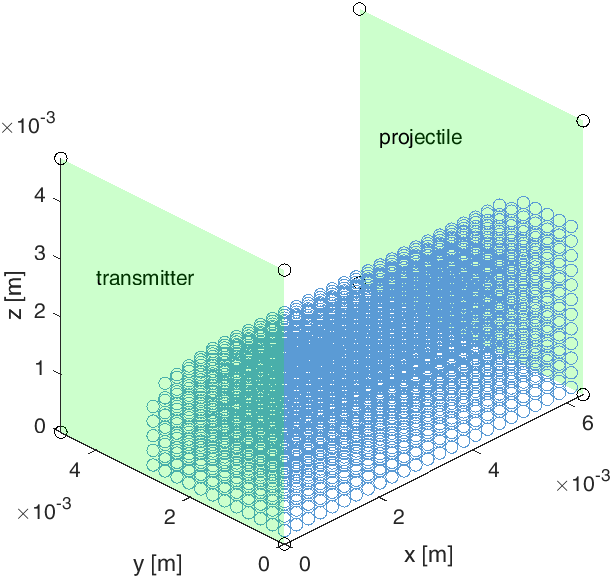
\includegraphics[width=6cm]{Figures/figure_setup.png}
\centering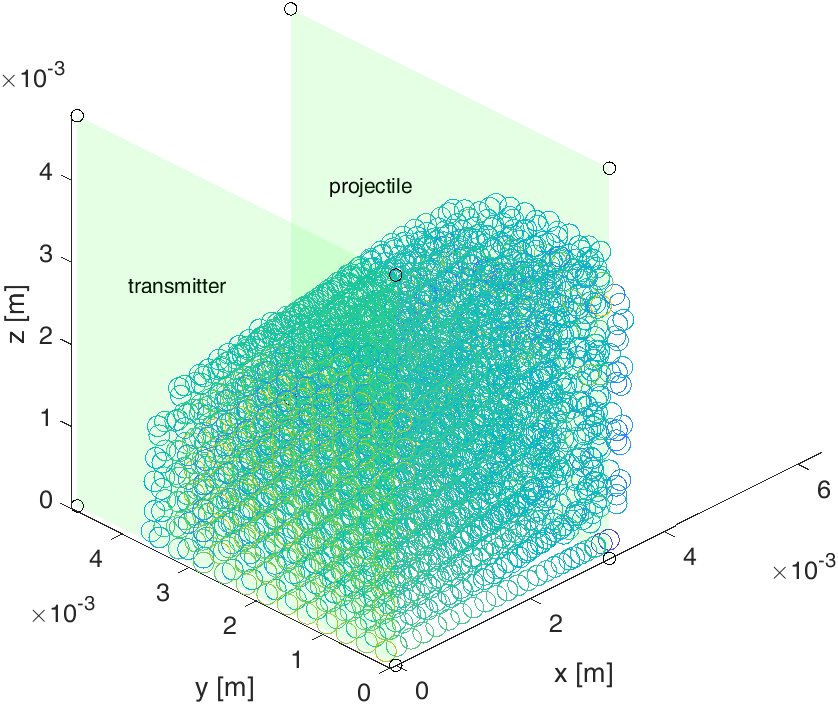
\includegraphics[width=6cm]{Figures/figure_compression.png}
\caption{Initial setup (left) and sample compression at $\epsilon=0.4$ (right)}
\label{fig:sample}
\end{figure}

Figure~\revb{\ref{fig:comparison}} compares the calculated stress-strain response to the experimentally achieved results (experimental data substracted from~\cite{Casem:2014}), where the stress is calculated as the ratio of the transmitter contact force and the cross-sectional area.

\begin{figure}
\centering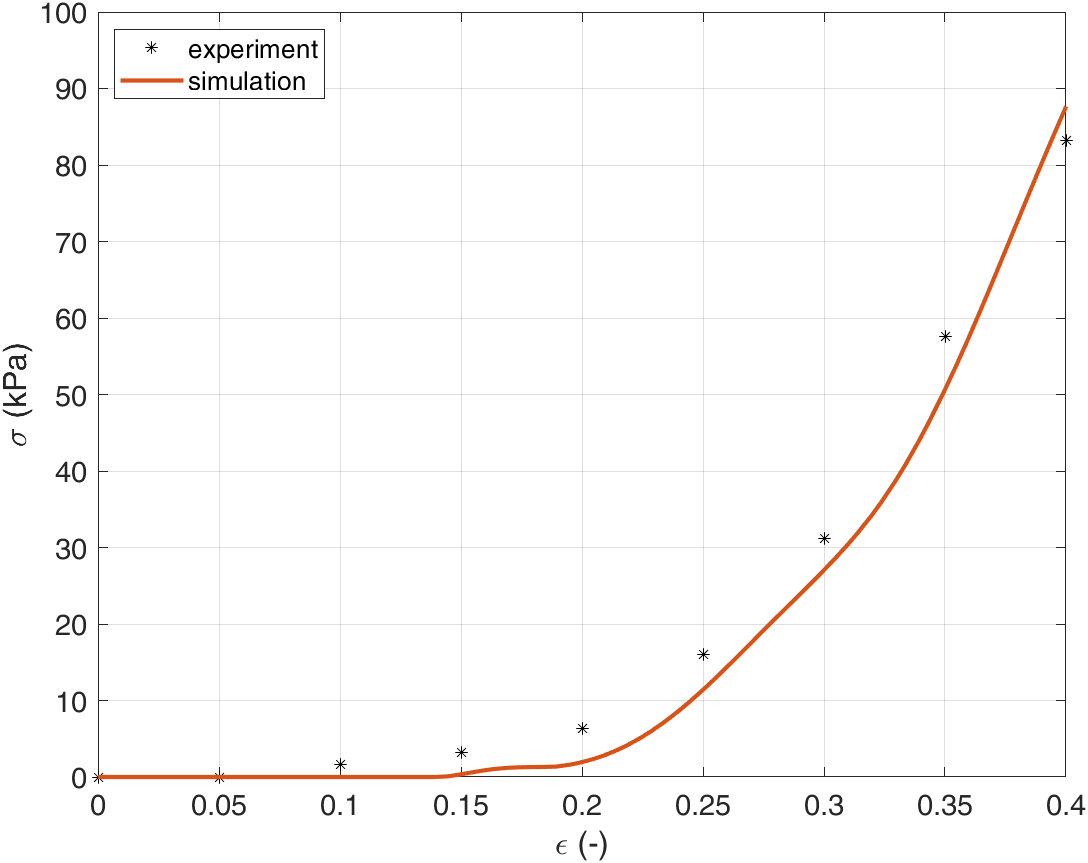
\includegraphics[width=6cm]{Figures/figure_comparison.png}
\caption{Stress-strain response}
\label{fig:comparison}
\end{figure}

The implemented material model shows a good response in high-speed compression for the given data. The ramp of the stress is a little bit slower, which can be caused by the slower wave propagation in the sample, which can also reflect in the higher final stress. Additional work is needed to tune the constitutive material properties for wider range of impacts.
%
\section{Conclusion}
%
The smoothed particle hydrodynamic with the solid dynamics in combination with the Mie-Gr\"uneisen equation of state was implemented for the numerical modelling of the ballistic gelatine with the material properties obtained from literature. Numerical simulations verified the response of the implemented ballistic gelatine material model under the high-speed compressions loading by comparing the simulation output to the experimental data. Therefore, smoothed particle hydrodynamics seems to be a promising method for modelling ballistic gelatine.
%
\section*{Acknowledgment}
%
This research was funded by the European Regional Development Fund-Project grant number CZ.02.1.01/0.0/0.0/17\_048/0007280.
%
\begin{thebibliography}{6}
%
\bibitem{Awoukeng:2014}
Awoukeng-Goumtcha, A., Taddei, L., Tostain, F., Roth, S.: Investigations of impact biomechanics for penetrating ballistic cases. Bio-Medical Materials and Engineering 24, 2331-2339 (2014).
\url{doi:10.3233/BME-141046}
%
\bibitem{Yoon:2015}
Yoon, G.H., Mo, J.S., Kim, K.H., Yoon, C.H., Lim, N.H.: Investigation of bullet penetration in ballistic gelatin via finite element simulation and experiment. Journal of Mechanical Science and Technology 29(9), 3747-3759 (2015).
\url{doi:10.1007/s12206-015-0821-7}
%
\bibitem{Chen:2020}
Chen, F., Chen, R., Jiang, B.: The adaptive finite element material point method for simulation of projectiles penetrating into ballistic gelatin at high velocities. Engineering Analysis with Boundary Elements117, 143-156 (2020).
\url{doi:10.1016/j.enganabound.2020.03.022}
%
\revb{
\bibitem{Subhash:2012}
Subhash, G., Kwon, J., Mei, R., Moore, D.F., Non-Newtonian Behavior of Ballistic Gelatin
at High Shear Rates. Experimental Mechanics 52, 551–560 (2012).
}
%
\bibitem{Taddei:2015}
Taddei, L., Awoukeng-Goumtcha, A.A., Roth, S.: Smoothed particle hydrodynamics formulation for penetrating impacts on ballistic gelatine. Mechanics Research Communications 90, 94-101 (2015).
\url{doi:10.1016/j.mechrescom.2015.09.010}
%
\bibitem{Frissane:2019}
Frissane, H., Taddei, L., Lebaal, N., Roth, S.: SPH modeling of high velocity impact into ballistic gelatin. Development of an axis-symmetrical formulation. Mechanics of Advanced Materials and Structures 26, 1881-1888 (2019)
\url{doi:10.1080/15376494.2018.1452322}
%
\bibitem{Khalil:2019}
Khalil, M.A., Frissane, H., Taddei, L., Meng, S., Lebaal, N., Demoly, F., Bir, C., Roth, S.: SPH-based method to simulate penetrating impact mechanics into ballistic gelatin: Toward an understanding of the perforation of human tissue. Extreme Mechanics Letters 29, 1-8 (2019).
\url{doi:10.1016/j.eml.2019.100479}
%
\bibitem{Gingold:1977}
Gingold, R.A., Monaghan, J.J.: Smoothed particle hydrodynamics: theory and application to non-spherical stars. Monthly Notices of the Royal Astronomical Society 181, 375-389 (1977). 
\url{doi:10.1093/mnras/181.3.375}
%
\bibitem{Lucy:1977}
Lucy, LB.: A numerical approach to the testing of the fission hypothesis. Astronomical Journal 82, 1013-1024 (1977). 
\url{doi:10.1086/112164}
%
\bibitem{Hyncik:2015}
Hyn\v{c}\'{\i}k, L.: SPHCOFEM: Solver for Coupling SPH and FE. IFMBE Proceedings 52, 162-165 (2015). 
\url{doi:10.1007/978-3-319-19452-3_43}
%
\bibitem{Hyncik:2022}
Hyn\v{c}\'{\i}k, L.: On modelling ballistic gelatine by smoothed particle hydrodynamics. In: 9$^{\mbox{\scriptsize th}}$ International Conference on Mechanics and Materials in Design, pp. 157-162. INEGI-FEUP (2022).
%
\bibitem{SPHCOFEM}
SPHCOFEM. \url{https://github.com/SPHCOFEM}
%
\bibitem{Ellero:2007}
Ellero, M., Serrano, M., Español, P.: Incompressible smoothed particle hydrodynamics. Journal of Computational Physics 226, 1731-1752 (2007). 
\url{doi:https://doi.org/10.1016/j.jcp.2007.06.019}
%
\bibitem{Monaghan:2006}
Monaghan, J.J.: Smoothed particle hydrodynamic simulations of shear flow. Monthly Notices of the Royal Astronomical Society 365, 199-213, (2006).
\url{doi:10.1111/j.1365-2966.2005.09704.x}
%
\bibitem{Czerner:2015}
Czerner, M., Sanchez Fellay, L., Su\'arez, M.P., Frontini, P.M., Fasce, L.A.: Determination of Elastic Modulus of Gelatin Gels by Indentation Experiments. Procedia Materials Science 8, 2211-8128 (2015)
\url{doi:10.1016/j.mspro.2015.04.075}
%
\bibitem{Robinson:2019}
Robinson, A.C.: The Mie-Grüneisen Power Equation of State. Sandia National Laboratories Technical Report (2019).
%
\bibitem{Casem:2014}
Casem, D.T., Dwivedi, A.K., Mrozek, R.A., Lenhart, J.L.: Compression response of a thermoplastic elastomer gel tissue surrogate over a range of strain-rates. International Journal of Solids and Structures 51, 2037-2046 (2014). 
\url{doi:10.1016/j.ijsolstr.2013.12.028}
%
\bibitem{Cygwin}
Cygwin. \url{http://www.cygwin.com}
%
%
\bibitem{MATLAB}
MATLAB, R2020a. \url{https://www.mathworks.com}
%
\bibitem{Dominguez:2011}
Dom\'{\i}nguez, J.M., Crespo, A.J.C., G\'omez-Gesteira, M., Marongiu, J.C.: Neighbour lists in smoothed particle hydrodynamics. International Journal for Numerical Methods in Fluids 67, 2026-2042 (2011).
\url{doi:10.1002/fld.2481}
%
\bibitem{Kolsky:1949}
Kolsky, H. An Investigation of the Mechanical Properties of Materials at Very High Rates of Loading. Proceedings of the Physical Society (Section B), 62, 676-700 (1949).
\url{doi:10.1088/0370-1301/62/11/302}
%
\bibitem{Hyncik:2002}
Hyn\v{c}\'{\i}k, L.: S Smoothed particle hydrodynamics: theory and practice. Engineering Mechanics 9, 1-15 (2002). 
%
%\bibitem{Becker:2007}
%Becker, M., Teschner, M.: Weakly compressible SPH for free surface flows. Eurographics / ACM SIGGRAPH Symposium on Computer Animation, pp. 1-8 (2007). 
%\url{doi:10.1145/1272690.1272719}

%\bibitem{Howe:2008}
%Howe, A.M., Pitt, A.R.: Rheology and stability of oil-in-water nanoemulsions stabilised by anionic surfactant and gelatin 1) addition of nonionic, cationic and ethoxylated-cationic co-surfactants. Advances in Colloid and Interface Science 2, 24-29 (2008). 
%\url{doi:10.1016/j.cis.2008.08.003}

%\bibitem{Subash:2012}
%Subhash, G., Kwon, J., Mei, R., Moore, D.F.: Non-Newtonian Behavior of Ballistic Gelatin at High Shear Rates. Experimental Mechanics 52, 551-560 (2012). 
%\url{doi:10.1007/s11340-011-9513-0}

%\bibitem{Yang:2009}
%Yang, H., Wang, Y.: Effects of concentration on nanostructural images and physical properties of gelatin from channel catfish skins. Food Hydrocoll 23, 577-584 (2009). 
%\url{doi:10.1016/j.foodhyd.2008.04.016}

%\bibitem{Veysset:2020}
%Veysset, D., Sun, Y., Lem, J., Kooi, S.E., Maznev, A.A., Cole, S.T., Mrozek, R.A., Lenhart, J.L., Nelson, K.A.: High-Strain-Rate Behavior of a Viscoelastic Gel Under High-Velocity Microparticle Impact. Experimental Mechanics 60, 1179-1186 (2020).
%\url{doi:10.1007/s11340-020-00639-9}
%
\end{thebibliography}
\end{document}
